% ============================================================
% LLM-BLM 実験 4：FinBERT の追加学習と LLM の比較
% コンパイル：tectonic -X compile LLM-BLM_実験4.tex   （XeTeX 系。このフォルダで実行する）
% 図は 図/（作成スクリプト/figs.py が DB と experiments/E4_finbert_finetune/results から作る）
% 数値の出どころは experiments/E4_finbert_finetune/results/summary.json と findings.md、
% 事前登録は experiments/E4_finbert_finetune/preregistration.md
% ============================================================
\documentclass[xelatex,ja=standard,jafont=haranoaji,a4paper,10pt,openany]{bxjsreport}
\setpagelayout*{left=24mm,right=24mm,top=24mm,bottom=26mm,footskip=11mm}

\usepackage{amsmath,amssymb,mathtools,bm}
\usepackage{booktabs,array,multirow,longtable}
\usepackage{graphicx}
\usepackage{adjustbox}
\usepackage{xcolor}
\usepackage{tikz}
\usetikzlibrary{arrows.meta,positioning,calc,fit}
\usepackage{enumitem}
\usepackage{caption}
\usepackage{float}
\usepackage[most]{tcolorbox}
\usepackage[hidelinks,bookmarksnumbered]{hyperref}
\pdfstringdefDisableCommands{\def\Omega{Ω}\def\tau{τ}\def\Sigma{Σ}}

\graphicspath{{図/}}

\definecolor{c1}{HTML}{2A78D6}
\definecolor{c2}{HTML}{EB6834}
\definecolor{c3}{HTML}{1BAF7A}
\definecolor{c4}{HTML}{EDA100}
\definecolor{c7}{HTML}{6250D6}
\definecolor{ink2}{HTML}{52514E}
\definecolor{soft1}{HTML}{E4EEF9}
\definecolor{soft2}{HTML}{FBEEDF}
\definecolor{soft3}{HTML}{E3F3E9}
\definecolor{soft4}{HTML}{EEE8FA}
\definecolor{soft5}{HTML}{FDF3DA}

\newcommand{\code}[1]{\texttt{#1}}
\newcommand{\SP}{S\&P500}
\newcommand{\figref}[1]{図~\ref{#1}}
\newcommand{\tabref}[1]{表~\ref{#1}}
\newcommand{\chapref}[1]{第~\ref{#1}~章}
\newcommand{\secref}[1]{\ref{#1}~節}

\setlist[itemize]{leftmargin=1.6em,itemsep=0.2em,topsep=0.4em}
\setlist[enumerate]{leftmargin=1.8em,itemsep=0.2em,topsep=0.4em}
\captionsetup{font=small,labelfont=bf,skip=6pt}
\renewcommand{\arraystretch}{1.2}
\setlength{\LTpre}{6pt}
\setlength{\LTpost}{6pt}

\makeatletter
\def\@makechapterhead#1{\vspace*{0.3\Cvs}{\parindent\z@\raggedright\normalfont
  \ifnum\c@secnumdepth>\m@ne\if@mainmatter{\Large\headfont\@chapapp\thechapter\@chappos}\par\nobreak\vskip0.4\Cvs\fi\fi
  \interlinepenalty\@M\LARGE\headfont #1\par\nobreak\vskip 1.5\Cvs}}
\def\@makeschapterhead#1{\vspace*{0.3\Cvs}{\parindent\z@\raggedright\normalfont
  \interlinepenalty\@M\LARGE\headfont #1\par\nobreak\vskip 1.5\Cvs}}
\makeatother

\newtcolorbox{keybox}[1][要点]{enhanced,breakable,colback=soft1,colframe=c1,boxrule=0.5pt,arc=2pt,
  left=8pt,right=8pt,top=6pt,bottom=6pt,title={#1},fonttitle=\sffamily\bfseries\small,coltitle=white}
\newtcolorbox{notebox}[1][注意]{enhanced,breakable,colback=soft2,colframe=c2,boxrule=0.5pt,arc=2pt,
  left=8pt,right=8pt,top=6pt,bottom=6pt,title={#1},fonttitle=\sffamily\bfseries\small,coltitle=white}
\newtcolorbox{verdict}[1][判定]{enhanced,breakable,colback=soft4,colframe=c7,boxrule=0.5pt,arc=2pt,
  left=8pt,right=8pt,top=6pt,bottom=6pt,title={#1},fonttitle=\sffamily\bfseries\small,coltitle=white}

\tikzset{
  box/.style={draw=#1,fill=#1!8,rounded corners=2pt,align=center,font=\footnotesize,inner sep=4pt,
              minimum height=10mm,text width=24mm},
  arr/.style={-{Stealth[length=2mm]},color=ink2,line width=0.6pt},
}

\title{LLM-BLM 実験 4\\[6pt]
  \large LLM の学習なしの読み取りは、\\過去の反応で追加学習した FinBERT を超えるか}
\author{実験の結果の報告書}
\date{2026 年 10 月 18 日}

\begin{document}
\maketitle

% ============================================================
\chapter*{概要}
\addcontentsline{toc}{chapter}{概要}

実験 2・3 で、gpt-4o-mini が決算発表文から読み取った点数（学習なし）は、発表への 2 取引日の反応を、辞書・FinBERT・TF-IDF・数値の驚き・アナリスト予想との差を超えて説明した。ただし、比べた相手のうち実際の反応で学習したのは、単語の出方を使う TF-IDF だけだった。今回は、文脈を読める FinBERT を、2015〜2022 年の決算発表の実際の反応で追加学習（深層学習）させ、LLM と比べた。手順・学習の設定・判定の基準は、学習の前に文書とコードで固定した（事前登録）。

\begin{keybox}[主な結論]
\begin{itemize}
\item \textbf{LLM の点数は、追加学習した FinBERT に置き換えられない（支持）。}追加学習した FinBERT と同時に入れても、LLM の係数は 1 標準偏差あたり $+102$bp（$t$ 7.8、置換の対照で $p=0.001$）で、実験 3 の $+116$bp の 88\% が残った。
\item \textbf{追加学習は効いた。}追加学習した FinBERT だけでも $+71$bp（$t$ 6.4）で、学習なしの FinBERT（$+39$bp）を大きく上回った。LLM と同時でも $+34$bp（$t$ 3.0）が残る。
\item \textbf{説明力は LLM が約 2.4 倍。}統制に加えたときの決定係数の増分は、LLM が $+2.01$ ポイント、追加学習した FinBERT が $+0.84$ ポイント。LLM に FinBERT を足しても $+0.17$ ポイントしか増えない。
\end{itemize}
\end{keybox}

\textbf{意味}：過去の反応で「当て方」を学ばせた専用のモデルより、学習なしの gpt-4o-mini のほうが、決算発表文から市場の受け取り方をよく読み取った。ただし、FinBERT が読むのは先頭の 512 トークンで、gpt-4o-mini は先頭の 15,000 字を読んでいる。差の一部は、読む量の差かもしれない。

\setcounter{tocdepth}{1}
{\small\tableofcontents}

% ============================================================
\chapter{目的}\label{ch:intro}

これまでの比べる相手は、次の 2 種類だった。
\begin{itemize}
\item \textbf{学習なしの文章の分析}：辞書（Loughran--McDonald）と FinBERT（語調の分類）。
\item \textbf{反応で学習した、単語の出方のモデル}：TF-IDF ＋ リッジ回帰。
\end{itemize}

「LLM でないとできない」と言うには、文脈を読める言語モデルを、同じ目的（発表への反応）で学習させた相手にも勝つ必要がある。深層学習で見込みがあるのは、株価の数値の予測ではなく、この「文章から反応」への学習である。実験 2 で、文章には反応を説明する情報がはっきりあると分かったからである。

\begin{verdict}[問い]
LLM（gpt-4o-mini）の学習なしの読み取りは、過去の反応で追加学習した FinBERT を超える情報を持つか。
\end{verdict}

% ============================================================
\chapter{方法と事前登録}\label{ch:method}

事前登録の文書（\code{experiments/E4\_finbert\_finetune/preregistration.md}）と学習・評価のコード（\code{run.py}）を、コミット \code{3c8f0db} に固定してから、1 回だけ実行した。

\section{学習}

\begin{table}[H]
\centering
\caption{追加学習の設定（事前登録で固定し、選び直していない）。}
\small
\begin{tabular}{lp{10.4cm}}
\toprule
元のモデル & \code{yiyanghkust/finbert-tone}（実験 2 の FinBERT と同じ版）。分類の頭を外し、出力 1 つの回帰の頭を付けた \\
事前学習の文章 & 論文によれば、10-K・10-Q は 1994〜2019 年、決算説明会は 2004〜2019 年、アナリストのレポートは 1995〜2008 年。評価期間（2023 年 11 月以降）より前 \\
入力 & 発表文の先頭 512 トークン \\
目的変数 & 2 取引日の超過リターン。学習の標本の 1\%・99\% 点で丸め、標準化 \\
学習の標本 & 提出日 2015〜2022 年の 13,979 本（評価の標本と重ならない） \\
設定 & AdamW、学習率 $2\times10^{-5}$、2 エポック、バッチ 16、最初の 10\% で学習率を上げてその後は直線で下げる、bf16、乱数の種 0。検証用の分割と早期終了は使わない \\
時間 & この PC の GPU（RTX 5050 Laptop）で 756 秒（1,748 歩） \\
予測 & 2023 年以降の 7,524 本。DB に点数の付け方の 1 つ（番号 8、反応を使う）として保存 \\
\bottomrule
\end{tabular}
\end{table}

\section{評価}

\begin{itemize}
\item \textbf{標本}：実験 3 と同じ標本 A（2023 年 11 月〜2026 年 8 月、5,374 本）。実験 2・3 で一度見た期間の再利用である。
\item \textbf{主な検定（モデル M2）}：実験 3 のモデル M1（実験 2 の統制＋アナリスト予想との差）に、追加学習した FinBERT の予測を加え、LLM の合成点数の係数を見る。t 検定（発表日ごとにまとめた標準誤差）と、同じ発表日の中での置換 1,000 回の両方で片側 $p<0.05$ なら「支持」。
\item \textbf{副次（Holm）}：S1 追加学習した FinBERT だけの係数、S2 LLM と同時の FinBERT の係数。
\item \textbf{説明力の比較}：統制に、LLM だけ・FinBERT だけ・両方を加えたときの決定係数の増分。
\end{itemize}

\begin{notebox}[解釈の注意（学習の前に事前登録に追記）]
LLM と追加学習した FinBERT が、同じ情報をそれぞれ誤差つきで測っている場合も、両方の係数が残る（作ったデータで確かめた）。そのため、「LLM の係数が残った」だけでは、LLM が独自の情報を持つとまでは言わない。「追加学習した FinBERT では置き換えられない」と書き、説明力の比較を並べて報告する。
\end{notebox}

% ============================================================
\chapter{結果}\label{ch:result}

\section{主な検定}

\begin{verdict}
\textbf{支持。}M2 の LLM の合成点数の係数は、1 標準偏差あたり $+102$bp（95\% 区間 $+77$〜$+128$bp、$t=7.77$）。置換の対照の片側 $p=0.001$。
\end{verdict}

\begin{figure}[H]
\centering
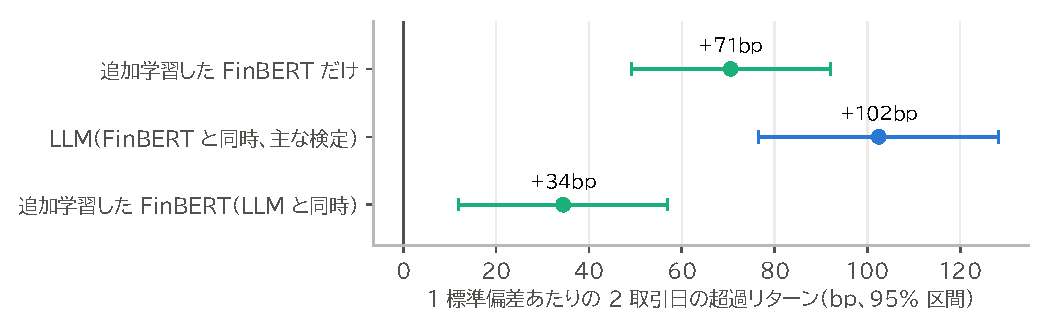
\includegraphics[width=0.92\linewidth]{coefficients.pdf}
\caption{追加学習した FinBERT と LLM の係数（1 標準偏差あたり、95\% 区間）。統制は実験 3 のモデル（アナリスト予想との差を含む）。}
\label{fig:coef}
\end{figure}

\begin{table}[H]
\centering
\caption{副次の分析（Holm で 2 つを補正）。}
\small
\begin{tabular}{lrrr}
\toprule
& 係数 & $t$ & Holm の $p$ \\
\midrule
S1 追加学習した FinBERT だけ（LLM なし） & $+71$bp & 6.45 & $<0.001$ \\
S2 追加学習した FinBERT（LLM と同時） & $+34$bp & 3.01 & 0.001 \\
\bottomrule
\end{tabular}
\end{table}

追加学習は効いた。学習なしの FinBERT（実験 2 で $+39$bp）より、追加学習した FinBERT（$+71$bp）は大きく反応を説明した。それでも、LLM と同時に入れると LLM の係数のほうがずっと大きく（\figref{fig:coef}）、FinBERT は $+34$bp に縮んだ。

\section{説明力の比較}

\begin{figure}[H]
\centering
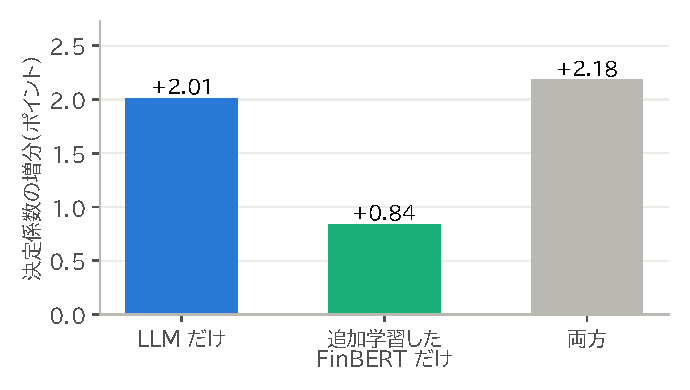
\includegraphics[width=0.6\linewidth]{r2_gain.pdf}
\caption{統制（実験 3 のモデルから LLM を除いたもの）に加えたときの、決定係数の増分。}
\label{fig:r2}
\end{figure}

LLM だけで $+2.01$ ポイント、追加学習した FinBERT だけで $+0.84$ ポイント、両方で $+2.18$ ポイントだった（\figref{fig:r2}）。
\begin{itemize}
\item FinBERT に LLM を足すと、$+1.34$ ポイント上乗せされる。
\item LLM に FinBERT を足しても、$+0.17$ ポイントしか上乗せされない。
\end{itemize}
2 つの点数の順位相関は 0.51 で、似ているが同じではない。LLM は、追加学習した FinBERT の持つ情報をほぼ含み、さらに多くを持つ側にある。

\section{2 つの点数の組み合わせ（探索）}

\begin{figure}[H]
\centering
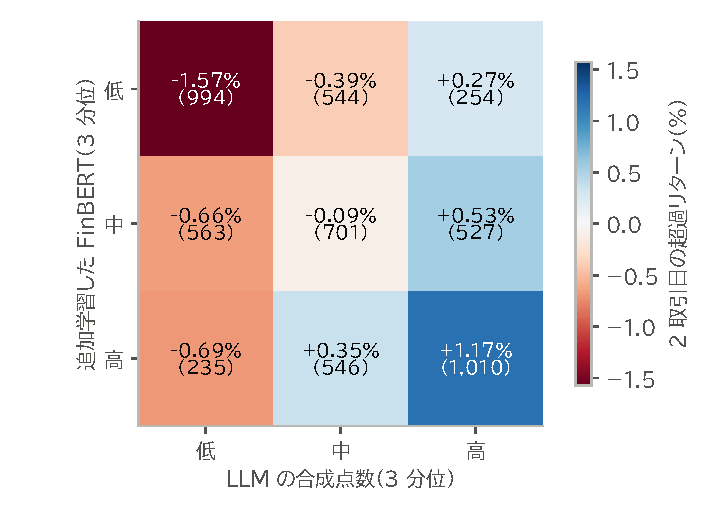
\includegraphics[width=0.62\linewidth]{double_sort.pdf}
\caption{LLM の合成点数と、追加学習した FinBERT の予測の 3 分位ごとの、2 取引日の超過リターンの平均（上下 1\% で丸め、括弧は本数）。探索の図で、判定には使っていない。}
\label{fig:double}
\end{figure}

FinBERT の 3 分位を固定して LLM を低から高に動かすと、どの行でも反応が 1.2〜1.9 ポイント上がる。逆に LLM を固定して FinBERT を動かしたときの差は 0.7〜0.9 ポイントで、小さい（\figref{fig:double}）。両方が高い発表は $+1.17\%$、両方が低い発表は $-1.57\%$ だった。

\section{頑健性}

\begin{itemize}
\item \textbf{R1}（アナリスト予想を除いた実験 2 の統制）：LLM $+105$bp（$t$ 7.75）、追加学習した FinBERT $+38$bp（$t$ 3.3）。
\item \textbf{R2}（すべて順位の版）：LLM は $t$ 5.69 で残り、追加学習した FinBERT は $t$ 1.1 で有意でなくなった。
\end{itemize}

% ============================================================
\chapter{考察と限界}\label{ch:discussion}

\section{何が分かったか}

過去の実際の反応で「当て方」を学ばせた専用のモデルより、学習なしの gpt-4o-mini のほうが、決算発表文から市場の受け取り方をよく読み取った。追加学習した FinBERT は、学習なしの FinBERT よりはっきり良くなったので、学習が失敗したわけではない。深層学習で反応の当て方を学ばせても、汎用の LLM の文章の理解には届かなかった、と読める。

\section{限界}

\begin{itemize}
\item \textbf{読む量が揃っていない。}FinBERT は先頭の 512 トークン（およそ 2,000〜2,500 字）、gpt-4o-mini は先頭の 15,000 字を読んでいる。見通しやガイダンスの節が後ろにある発表では、FinBERT は読めていない。段落ごとに予測して平均するなど、読む量を揃えた比較が残っている。
\item \textbf{学習の設定は 1 つだけ。}事前登録で固定した。もっと良い設定はありうるが、評価の結果を見て選び直すと過剰適合になる。
\item \textbf{取引の価値は別の話。}反応は 2 日で出尽くす（実験 2・3）。この実験は「どちらがよく読めるか」の比較で、儲けにつながるかは扱っていない。
\item \textbf{標本 A は、実験 2・3 で一度見た期間}である。
\end{itemize}

% ============================================================
\chapter*{再現の手順}
\addcontentsline{toc}{chapter}{再現の手順}

\begin{verbatim}
python experiments/E2_event_reaction/run.py   # 実験 2 の panel.csv
python experiments/E4_finbert_finetune/run.py    # 学習・予測・評価
cd 資料集/02_実験/実験4_FinBERT追加学習
python 作成スクリプト/figs.py                      # この資料の図
\end{verbatim}

数値の出どころは \code{experiments/E4\_finbert\_finetune/results/summary.json} と \code{findings.md}。費用は 0 円（この PC の GPU）。

\end{document}
